\chapter{Describir un sistema químico: avance, actividades, Q y K}\label{ch:b1:extent-q-and-k}

Una planta de hidrógeno introduce gas natural y vapor de agua en tubos
calentados al rojo; lo que sale nunca es hidrógeno puro, sino una mezcla
de hidrógeno, monóxido de carbono, dióxido de carbono, metano sin
reaccionar y vapor, cuyas proporciones deben conocer los ingenieros antes
de diseñar la unidad siguiente. Predecir la composición que sale de un
reactor --- el estado final de un sistema químico --- es el objeto de
este capítulo. Para ello hacen falta una descripción precisa del sistema
(sus variables y su composición), un único número que mida hasta dónde
ha llegado una reacción (el avance) y la ley que dice dónde se detiene la
reacción (la constante de equilibrio). Estas herramientas se usan en
todos los capítulos posteriores sobre disoluciones.

\begin{recall}
El libro 1 (año 10) siguió una reacción con una tabla de avance y halló
el \omterm{def:b1:extent-q-and-k:max-extent}{reactivo limitante}; el libro 1 (año 12) introdujo el \omterm{def:b1:extent-q-and-k:quotient}{cociente de
reacción} $Q$ y la constante de equilibrio $K$ de una reacción no total.
De la física se usa la ley de los gases perfectos, $pV = nRT$, con $R =
\qty{8.314}{J/(mol.K)}$.
\end{recall}

\begin{omfigure}
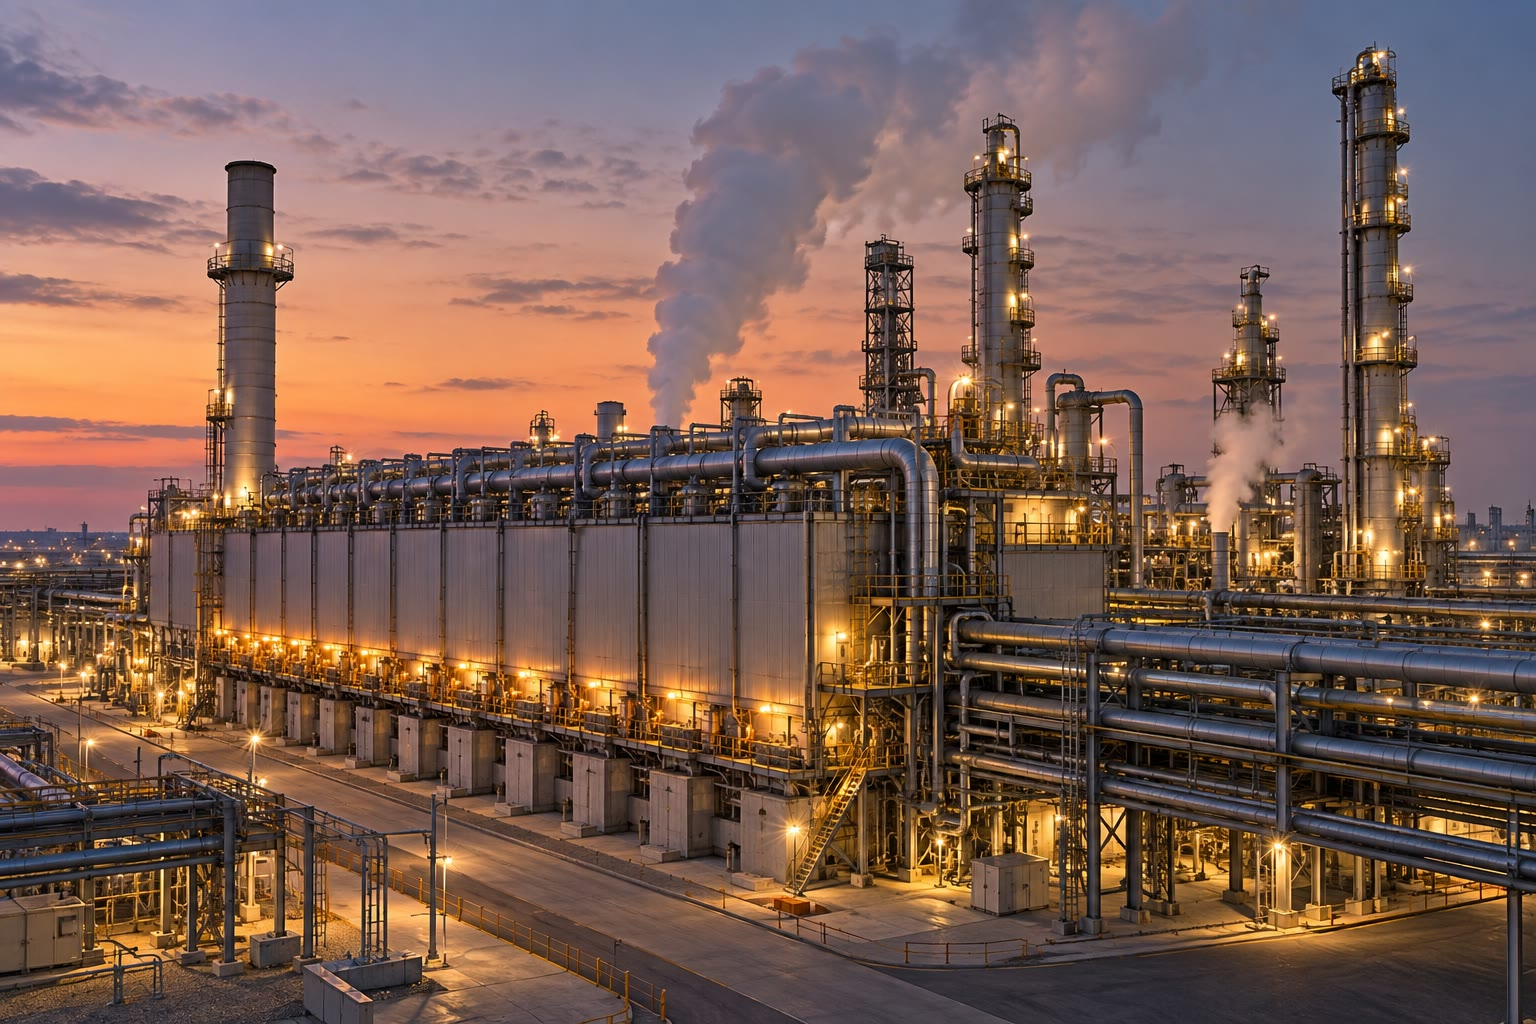
\includegraphics[width=0.6\linewidth]{images/book2/ai/b1-07-hydrogen-plant.jpg}

{\small Una planta de hidrógeno al anochecer. El gas natural y el vapor
reaccionan en el largo horno de reformado; un segundo reactor convierte
el monóxido de carbono; la composición a la salida es un estado final
del tipo que se calcula en este capítulo.}
\end{omfigure}

\section{Describir un sistema}

\begin{definition}[Sistema, fase]\label{def:b1:extent-q-and-k:system}
Un \emph{sistema fisicoquímico}\index{sistema fisicoquimico@sistema fisicoquímico} es la materia
contenida en una región del espacio elegida; el resto es su entorno. Es
un \emph{sistema cerrado}\index{sistema cerrado} si no intercambia materia
con el entorno (puede intercambiar energía). Una \emph{fase}\index{fase}
es una parte del sistema en la que las \omterm{def:b1:extent-q-and-k:variables}{variables intensivas} varían de
forma continua: una mezcla de gases es una sola fase; dos líquidos
inmiscibles son dos fases; cada sólido es una fase por sí mismo.
\end{definition}

\begin{definition}[Variables intensivas y extensivas]\label{def:b1:extent-q-and-k:variables}
Una variable de estado es \emph{extensiva}\index{variable extensiva} si es
proporcional al tamaño del sistema (masa, volumen, cantidad de sustancia)
e \emph{intensiva}\index{variable intensiva} si no lo es (temperatura,
presión, concentración, densidad, \omterm{def:b1:extent-q-and-k:composition}{fracción molar}). El cociente de dos
variables extensivas es intensivo.
\end{definition}

\begin{definition}[Variables de composición]\label{def:b1:extent-q-and-k:composition}
Para un constituyente $i$ de una \omterm{def:b1:extent-q-and-k:system}{fase} que contiene las cantidades $n_j$
de todos sus constituyentes:
\begin{itemize}
  \item su \emph{fracción molar}\index{fraccion molar@fracción molar} es $x_i = n_i/\sum_j
        n_j$, y su \emph{fracción másica}\index{fraccion masica@fracción másica} $w_i =
        m_i/\sum_j m_j$; ambas están entre 0 y 1 y suman 1;
  \item en una disolución de volumen $V$, su \emph{concentración
        molar}\index{concentracion molar@concentración molar} es $c_i = [i] = n_i/V$,
        en \unit{mol/L};
  \item en una mezcla de gases a la presión total $p$, su \emph{presión
        parcial}\index{presion parcial@presión parcial} es $p_i = x_i\,p$.
\end{itemize}
\end{definition}

\begin{proposition}[Presiones parciales de los gases perfectos]\label{prop:b1:extent-q-and-k:dalton}
En una mezcla de gases perfectos de volumen $V$ a la temperatura $T$, la
\omterm{def:b1:extent-q-and-k:composition}{presión parcial} de un constituyente es la presión que ejercería él solo
en todo el volumen, $p_i = n_iRT/V$, y las \omterm{def:b1:extent-q-and-k:composition}{presiones parciales} suman la
presión total: $\sum_i p_i = p$.
\end{proposition}

\begin{proof}
Para la mezcla, $pV = (\sum_j n_j)RT$, de modo que $p_i = x_i p = \frac{n_i}{\sum_j
n_j}\cdot\frac{(\sum_j n_j)RT}{V} = \frac{n_iRT}{V}$, y $\sum_i x_i = 1$
da $\sum_i p_i = p$.
\end{proof}

\begin{example}[El aire]\label{ex:b1:extent-q-and-k:air}
El aire seco contiene, en volumen (es decir, en cantidad, para gases
perfectos), un 78.08\,\% de dinitrógeno, un 20.95\,\% de dioxígeno y un
0.93\,\% de argón. A \qty{1.013}{bar}, la \omterm{def:b1:extent-q-and-k:composition}{presión parcial} del dioxígeno es
$0.2095 \times
1.013 = \qty{0.212}{bar}$; en una montaña donde la presión es de
\qty{0.70}{bar}, baja a \qty{0.147}{bar}, aunque la composición sea la
misma.
% ledger: air:N2, air:O2, air:Ar, const:atm
\end{example}

\section{Avance de la reacción}

\begin{definition}[Números estequiométricos, avance]\label{def:b1:extent-q-and-k:extent}
Una reacción se escribe $0 = \sum_i \nu_i\,\mathrm{A}_i$, donde el
\emph{número estequiométrico}\index{numero estequiometrico@número estequiométrico} $\nu_i$ de
la especie $\mathrm{A}_i$ es negativo para un reactivo y positivo para un
producto: en \ce{N2 + 3H2 -> 2NH3}, $\nu(\ce{N2}) = -1$, $\nu(\ce{H2}) = -3$,
$\nu(\ce{NH3}) = +2$. En un \omterm{def:b1:extent-q-and-k:system}{sistema cerrado} en el que solo tiene lugar
esta reacción, las cantidades varían según
\[
  n_i = n_{i,0} + \nu_i\,\xi ,
\]
lo que define el \emph{avance de la reacción}\index{avance de la reaccion@avance de la reacción}
$\xi$ (en moles), nulo al principio e igual para todas las especies.
\end{definition}

\begin{definition}[Avance máximo, reactivo limitante]\label{def:b1:extent-q-and-k:max-extent}
El \emph{avance máximo}\index{avance maximo@avance máximo} $\xi_{\max}$ es el mayor valor
de $\xi$ para el que ninguna cantidad es negativa: $\xi_{\max} = \min_{\nu_i <
0} n_{i,0}/|\nu_i|$. El reactivo que llega a cero en $\xi_{\max}$ es el
\emph{reactivo limitante}\index{reactivo limitante}. Cuando el avance puede
ser también negativo (reacción inversa), $\xi_{\min} = -\min_{\nu_i > 0}
n_{i,0}/\nu_i$.
\end{definition}

\begin{method}[La tabla de avance]\label{met:b1:extent-q-and-k:progress-table}
Para seguir una reacción en un \omterm{def:b1:extent-q-and-k:system}{sistema cerrado}:
\begin{enumerate}
  \item se escribe la ecuación ajustada y, debajo, una columna por
        especie;
  \item primera fila: las cantidades iniciales $n_{i,0}$;
  \item segunda fila: las cantidades en el avance $\xi$, $n_{i,0} + \nu_i\xi$;
  \item para los gases, se añade una columna con la cantidad total
        $n_{\text{tot}}(\xi)$;
  \item se calcula $\xi_{\max}$ (y $\xi_{\min}$) y se identifica el
        \omterm{def:b1:extent-q-and-k:max-extent}{reactivo limitante};
  \item última fila: las cantidades finales, en el avance final $\xi_f$
        (hallado a partir de la condición de equilibrio, o igual a
        $\xi_{\max}$ si la reacción es total).
\end{enumerate}
\end{method}

\begin{example}[Síntesis del amoniaco]\label{ex:b1:extent-q-and-k:ammonia}
A partir de \qty{2.0}{mol} de \ce{N2} y \qty{3.0}{mol} de \ce{H2}:
\begin{center}
\begin{tabular}{lcccc}
\hline
 & \ce{N2} & \ce{3H2} & \ce{2NH3} & total \\
\hline
inicial & 2.0 & 3.0 & 0 & 5.0 \\
avance $\xi$ & $2.0 - \xi$ & $3.0 - 3\xi$ & $2\xi$ & $5.0 - 2\xi$ \\
\hline
\end{tabular}
\end{center}
$\xi_{\max} = \min(2.0/1,\ 3.0/3) = \qty{1.0}{mol}$: el dihidrógeno es el
limitante. Si la reacción fuera total, el estado final contendría
\qty{1.0}{mol} de \ce{N2} y \qty{2.0}{mol} de \ce{NH3}.
\end{example}

\begin{definition}[Grado de avance final, rendimiento]\label{def:b1:extent-q-and-k:fractional-extent}
El \emph{grado de avance final}\index{grado de avance final} de una
reacción es $\tau = \xi_f/\xi_{\max}$, comprendido entre 0 y 1. En una
síntesis, el \emph{rendimiento}\index{rendimiento} de un producto es el
cociente entre la cantidad obtenida y la que daría el \omterm{def:b1:extent-q-and-k:max-extent}{reactivo limitante}
si la reacción fuera total; cuando no se pierde producto durante su
aislamiento, es igual a $\tau$.
\end{definition}

\section{Actividades}

\begin{definition}[Estado estándar, actividad]\label{def:b1:extent-q-and-k:activity}
La \emph{actividad}\index{actividad} $a_i$ de una especie es un número
adimensional que mide, en la expresión de las leyes de equilibrio, cuánta
cantidad de ella está disponible; se define respecto de un \emph{estado
estándar}\index{estado estandar@estado estándar}, un estado de referencia a la temperatura
considerada y a la presión estándar $p^\circ = \qty{1}{bar}$. En las
aproximaciones ideales que se usan en este libro:
\begin{itemize}
  \item para un gas, $a_i = p_i/p^\circ$ (el estado estándar es el gas
        perfecto puro a $p^\circ$);
  \item para un soluto en una disolución diluida, $a_i = c_i/c^\circ$ con
        $c^\circ = \qty{1}{mol/L}$;
  \item para el disolvente de una disolución diluida, y para un sólido
        puro o un líquido puro solo en su \omterm{def:b1:extent-q-and-k:system}{fase}, $a_i = 1$.
\end{itemize}
\end{definition}
% ledger: const:pstd

\begin{remark}[Ideal y real]\label{rem:b1:extent-q-and-k:ideal}
Estas expresiones valen para los gases perfectos y para las disoluciones
diluidas. En las disoluciones concentradas, los iones se atraen y se
repelen, y la \omterm{def:b1:extent-q-and-k:activity}{actividad} se aparta de $c_i/c^\circ$; las correcciones,
escritas con coeficientes de \omterm{def:b1:extent-q-and-k:activity}{actividad}, se estudian en el volumen del
segundo año junto con el potencial químico. Para las concentraciones que
se usan en este libro (por debajo de unos \qty{0.1}{mol/L}), las
expresiones ideales son exactas a unos pocos por ciento.
\end{remark}

\section{El cociente de reacción y la constante de equilibrio}

\begin{definition}[Cociente de reacción]\label{def:b1:extent-q-and-k:quotient}
El \emph{cociente de reacción}\index{cociente de reaccion@cociente de reacción} de una reacción
$0 = \sum_i \nu_i\,\mathrm{A}_i$ en un estado dado del sistema es
\[
  Q = \prod_i a_i^{\nu_i} ,
\]
el producto de las \omterm{def:b1:extent-q-and-k:activity}{actividades} de los productos dividido por el de los
reactivos, cada una elevada a su coeficiente estequiométrico.
\end{definition}

\begin{example}[Tres cocientes]\label{ex:b1:extent-q-and-k:quotients}
Para \ce{N2(g) + 3H2(g) <=> 2NH3(g)}: $Q = \dfrac{(p_{\ce{NH3}}/p^\circ)^2}
{(p_{\ce{N2}}/p^\circ)(p_{\ce{H2}}/p^\circ)^3}$. Para
\ce{CH3COOH(aq) + H2O(l) <=> CH3COO^-(aq) + H3O+(aq)}: $Q =
\dfrac{[\ce{CH3COO-}][\ce{H3O+}]}{[\ce{CH3COOH}]\,c^\circ}$, pues el
disolvente tiene \omterm{def:b1:extent-q-and-k:activity}{actividad} 1. Para \ce{CaCO3(s) <=> CaO(s) + CO2(g)}: $Q =
p_{\ce{CO2}}/p^\circ$, pues los sólidos tienen \omterm{def:b1:extent-q-and-k:activity}{actividad} 1.
\end{example}

\begin{definition}[Constante de equilibrio estándar]\label{def:b1:extent-q-and-k:equilibrium-constant}
La \emph{constante de equilibrio estándar}\index{constante de equilibrio estandar@constante de equilibrio estándar}
$K^\circ$ de una reacción es el valor que toma su \omterm{def:b1:extent-q-and-k:quotient}{cociente de reacción}
cuando el sistema está en equilibrio. Es adimensional y solo depende de
la reacción y de la temperatura.
\end{definition}

\begin{theorem}[Ley de acción de masas]\label{thm:b1:extent-q-and-k:mass-action}
A una temperatura dada, un sistema en el que una reacción puede tener
lugar en los dos sentidos evoluciona hasta que $Q = K^\circ(T)$; en el
equilibrio, sea cual sea la composición inicial,
\[
  \prod_i a_{i,\text{eq}}^{\nu_i} = K^\circ(T) .
\]
\end{theorem}
\admitted

\begin{proposition}[Sentido de evolución]\label{prop:b1:extent-q-and-k:direction}
Un sistema en el que $Q < K^\circ$ evoluciona en sentido directo ($\xi$
aumenta); si $Q > K^\circ$, evoluciona en sentido inverso; si
$Q = K^\circ$, está en equilibrio.
\end{proposition}
\admitted

\begin{remark}[De dónde salen estas leyes]\label{rem:b1:extent-q-and-k:origin}
Ambos enunciados se deducen del segundo principio de la termodinámica, a
través de la entalpía libre de reacción y de los potenciales químicos de
las especies: se demuestran en el volumen del segundo año, que también da
$K^\circ$ a partir de tablas de datos termodinámicos y explica cómo
varía con la temperatura. Aquí se usan como leyes.
\end{remark}

\begin{omfigure}
\begin{tikzpicture}[font=\small, >={Stealth}]
  \draw[->, thick] (0,0) -- (11,0) node[right] {$Q$};
  \draw[thick, omThm] (5.5,0.25) -- (5.5,-0.25) node[below] {$K^\circ$};
  \draw[->, omDef, thick] (1.0,0.55) -- (4.6,0.55);
  \node[above, omDef] at (2.8,0.6) {$Q < K^\circ$: directo};
  \draw[->, omProp, thick] (10.0,0.55) -- (6.4,0.55);
  \node[above, omProp] at (8.2,0.6) {$Q > K^\circ$: inverso};
  \node[below] at (0,-0.1) {0};
\end{tikzpicture}

{\small El cociente se desplaza hacia la constante: un sistema con $Q <
K^\circ$ forma productos; uno con $Q > K^\circ$ los consume.}
\end{omfigure}

\begin{proposition}[Combinación de constantes]\label{prop:b1:extent-q-and-k:combine-k}
Si $K_1^\circ$ y $K_2^\circ$ son las constantes de las reacciones (1) y
(2): la inversa de (1) tiene la constante $1/K_1^\circ$; la reacción
$n \times
(1)$ tiene $(K_1^\circ)^n$; la suma $(1) + (2)$ tiene $K_1^\circ K_2^\circ$.
\end{proposition}

\begin{proof}
El cociente de la reacción inversa es $\prod a_i^{-\nu_i} = 1/Q_1$; el de
$n \times (1)$ es $\prod a_i^{n\nu_i} = Q_1^n$; el de la suma es
$\prod a_i^{\nu_{i,1} + \nu_{i,2}} = Q_1 Q_2$. Al escribir estas
identidades en el equilibrio, donde cada cociente es igual a su
constante, se obtiene el resultado.
\end{proof}

\begin{proposition}[Un único estado de equilibrio]\label{prop:b1:extent-q-and-k:q-monotone}
Para una sola reacción en un \omterm{def:b1:extent-q-and-k:system}{sistema cerrado} a temperatura fija (y, para
los gases, a volumen o presión fijos), el cociente $Q(\xi)$ es una
función estrictamente creciente de $\xi$ en $(\xi_{\min}, \xi_{\max})$,
que va de 0 a $+\infty$ cuando no interviene ninguna especie de
\omterm{def:b1:extent-q-and-k:activity}{actividad} constante. La ecuación $Q(\xi) = K^\circ$ tiene entonces
exactamente una solución en ese intervalo.
\end{proposition}

\begin{proof}
Sea una reacción en disolución, $Q(\xi) = \prod_i (n_{i,0} + \nu_i\xi)^{\nu_i}
\times \text{const}$. Su derivada logarítmica es
\[
  \frac{\dd \ln Q}{\dd \xi} = \sum_i \frac{\nu_i^2}{n_{i,0} + \nu_i \xi}
  > 0 ,
\]
pues cada término es positivo donde lo son todas las cantidades. Cuando
$\xi \to \xi_{\max}$, la cantidad de un reactivo tiende a 0 en un
denominador y $Q \to +\infty$; cuando $\xi
\to \xi_{\min}$, la cantidad de un producto tiende a 0 y $Q \to 0$. Una
función continua y creciente de 0 a $+\infty$ toma el valor $K^\circ$
una sola vez. (Para gases a presión constante, la cantidad total también
varía; el resultado sigue siendo válido, como puede comprobarse en cada
caso.)
\end{proof}

\section{Estados finales}

\begin{definition}[Estado de equilibrio, reacción cuantitativa]\label{def:b1:extent-q-and-k:quantitative}
El estado final es un \emph{estado de equilibrio}\index{estado de equilibrio}
cuando todas las especies de la reacción están presentes y $Q = K^\circ$.
La reacción es \emph{cuantitativa}\index{reaccion cuantitativa@reacción cuantitativa} (o total)
cuando en el estado final el \omterm{def:b1:extent-q-and-k:max-extent}{reactivo limitante} ha desaparecido
prácticamente, $\xi_f \approx \xi_{\max}$; esto ocurre cuando $K^\circ$
es muy grande.
\end{definition}

\begin{method}[Hallar el estado final]\label{met:b1:extent-q-and-k:final-state}
Para hallar el estado final de una sola reacción:
\begin{enumerate}
  \item se dibuja la tabla de avance y se calcula $\xi_{\max}$ (y
        $\xi_{\min}$);
  \item se calcula $Q$ al principio y se compara con $K^\circ$ para
        hallar el sentido;
  \item se expresa $Q(\xi)$ con las \omterm{def:b1:extent-q-and-k:activity}{actividades} y se resuelve
        $Q(\xi) = K^\circ$ para $\xi$ en $(\xi_{\min}, \xi_{\max})$;
  \item si interviene una especie de \omterm{def:b1:extent-q-and-k:activity}{actividad} 1 (un sólido), se
        comprueba que sigue presente en ese avance: si tuviera que volverse
        negativa, desaparece antes y el estado final \emph{no} es un
        equilibrio ($\xi_f = \xi_{\max}$, $Q_f \ne K^\circ$).
\end{enumerate}
\end{method}

\begin{method}[La hipótesis de reacción cuantitativa]\label{met:b1:extent-q-and-k:quantitative}
Cuando $K^\circ$ es grande (típicamente superior a $10^4$), se supone la
reacción total: se toma $\xi_f = \xi_{\max}$, se calculan las cantidades
finales y luego se halla la pequeña cantidad $\varepsilon$ de \omterm{def:b1:extent-q-and-k:max-extent}{reactivo
limitante} que queda escribiendo $Q =
K^\circ$ con las demás cantidades sin cambios. La hipótesis se acepta si
$\varepsilon$ es pequeña frente a las demás cantidades (por debajo de un
1\,\% aproximadamente).
\end{method}

\begin{example}[Una reacción cuantitativa]\label{ex:b1:extent-q-and-k:quant}
Para $\mathrm{A + B \rightleftharpoons C + D}$ en disolución con $[\ce{A}]_0 = [\ce{B}]_0 =
\qty{0.10}{mol/L}$ y $K^\circ = 10^6$: suponiendo la reacción total,
$[\ce{C}]
= [\ce{D}] = 0.10$; entonces, $0.10^2/\varepsilon^2 = 10^6$ da $\varepsilon
= \qty{1.0e-4}{mol/L}$, un 0.1\,\% de la cantidad inicial: la hipótesis
está justificada.
\end{example}

\begin{omfigure}
\begin{tikzpicture}
\begin{axis}[
  width=0.45\linewidth, height=5.6cm, ymode=log,
  xmin=0, xmax=1, ymin=0.01, ymax=1000,
  axis x line=bottom, axis y line=left,
  xlabel={avance $\xi$ (mol)}, ylabel={$Q$}, xtick={0,0.2,0.4,0.8,1},
  tick label style={font=\small}, label style={font=\small}, clip=false]
\addplot[omDef, thick] table[x=xi, y=Q] {figdata/out/bachelor-1-extent-equilibrium-shift.dat};
\draw[omThm, dashed] (axis cs:0,4) -- (axis cs:1,4);
\node[omThm, anchor=south west, font=\small] at (axis cs:0.02,4) {$K^\circ = 4.0$};
\draw[dotted] (axis cs:0.607,0.01) -- (axis cs:0.607,4);
\node[anchor=north, font=\small] at (axis cs:0.607,0.01) {0.607};
\end{axis}
\end{tikzpicture}\hfill
\begin{tikzpicture}
\begin{axis}[
  width=0.45\linewidth, height=5.6cm,
  xmin=0, xmax=0.04, ymin=0, ymax=0.3,
  axis x line=bottom, axis y line=left,
  xlabel={avance $\xi$ (mol)}, ylabel={$Q = p_{\ce{CO2}}/p^\circ$},
  xtick={0,0.01,0.02,0.03,0.04}, scaled x ticks=false,
  xticklabel style={/pgf/number format/fixed, /pgf/number format/precision=2},
  yticklabel style={/pgf/number format/fixed},
  tick label style={font=\small}, label style={font=\small}, clip=false]
\addplot[omProp, thick] table[x=xi, y=Q_small] {figdata/out/bachelor-1-extent-equilibrium-carbonate.dat};
\addplot[omDef, thick, dashed] table[x=xi, y=Q_large] {figdata/out/bachelor-1-extent-equilibrium-carbonate.dat};
\draw[omThm, dashed] (axis cs:0,0.2) -- (axis cs:0.04,0.2);
\node[omThm, anchor=south west, font=\small] at (axis cs:0.0005,0.2) {$K^\circ = 0.20$};
\node[omProp, anchor=north west, font=\scriptsize] at (axis cs:0.012,0.088) {\qty{0.010}{mol}: sólido agotado};
\node[omDef, anchor=north west, font=\scriptsize] at (axis cs:0.024,0.19) {\qty{0.050}{mol}: equilibrio};
\end{axis}
\end{tikzpicture}

{\small A la izquierda, el cociente de \ce{CO + H2O <=> CO2 + H2} crece
con el avance y alcanza $K^\circ$ una sola vez (problema de fin de
semana). A la derecha, para \ce{CaCO3(s) <=> CaO(s) + CO2(g)} en un
recipiente cerrado de \qty{10}{L},
$Q = p_{\ce{CO2}}/p^\circ$ crece con $\xi$; con \qty{0.050}{mol} de
carbonato alcanza $K^\circ = 0.20$ (equilibrio); con \qty{0.010}{mol}, el
carbonato se agota antes y el estado final no es un equilibrio.}
\end{omfigure}

\begin{method}[Dos reacciones simultáneas]\label{met:b1:extent-q-and-k:two-reactions}
Cuando dos reacciones tienen lugar en el mismo sistema, se asigna a cada
una su propio avance, $\xi_1$ y $\xi_2$; cada cantidad es $n_i = n_{i,0} + \nu_{i,1}\xi_1
+ \nu_{i,2}\xi_2$, y el estado final cumple a la vez $Q_1 = K_1^\circ$ y
$Q_2 = K_2^\circ$ (un sistema de dos ecuaciones). Si una constante es
mucho mayor que la otra, se trata primero la reacción correspondiente
como \omterm{def:b1:extent-q-and-k:quantitative}{cuantitativa} y, después, la segunda sobre el resultado.
\end{method}

\begin{history}[La ley de acción de masas, 1864]
En 1864, el químico noruego Cato Guldberg y su cuñado, el farmacéutico
Peter Waage, publicaron en noruego su ley de las ``masas activas'': una
reacción avanza hasta que se equilibran las fuerzas de las reacciones
directa e inversa, cada una proporcional a las concentraciones de sus
reactivos. Su trabajo pasó inadvertido en el extranjero hasta que lo
volvieron a publicar en dos lenguas más leídas, en 1867 y en 1879;
Jacobus van 't Hoff, que había redescubierto la ley, reconoció su
prioridad.
\end{history}

\section{Ejercicios}

\begin{exercise}[$\star$]\label{exo:b1:extent-q-and-k:1}
Clasifíquense en \omterm{def:b1:extent-q-and-k:variables}{intensivas} o \omterm{def:b1:extent-q-and-k:variables}{extensivas}: la temperatura, el volumen, la
cantidad de sustancia, la \omterm{def:b1:extent-q-and-k:composition}{concentración molar}, la densidad, la presión,
la masa y la \omterm{def:b1:extent-q-and-k:composition}{fracción molar}.
\end{exercise}

\begin{exercise}[$\star$]\label{exo:b1:extent-q-and-k:2}
Con la composición del aire seco dada en el capítulo, calcúlense las
\omterm{def:b1:extent-q-and-k:composition}{presiones parciales} de \ce{N2}, \ce{O2} y \ce{Ar} a una presión total de
\qty{1.013}{bar}.
\end{exercise}

\begin{exercise}[$\star$]\label{exo:b1:extent-q-and-k:3}
Dibújese la tabla de avance de \ce{2H2 + O2 -> 2H2O} a partir de
\qty{3.0}{mol} de \ce{H2} y \qty{2.0}{mol} de \ce{O2}. Hállense
$\xi_{\max}$, el \omterm{def:b1:extent-q-and-k:max-extent}{reactivo limitante} y el estado final si la reacción es
total.
\end{exercise}

\begin{exercise}[$\star$]\label{exo:b1:extent-q-and-k:4}
Escríbase el \omterm{def:b1:extent-q-and-k:quotient}{cociente de reacción} de: (a) \ce{CaCO3(s) <=> CaO(s) + CO2(g)};
(b) \ce{Ag+(aq) + Cl-(aq) <=> AgCl(s)}; (c) \ce{N2(g) + 3H2(g) <=>
2NH3(g)}; (d) \ce{NH3(aq) + H2O(l) <=> NH4+(aq) + OH-(aq)}.
\end{exercise}

\begin{exercise}[$\star\star$]\label{exo:b1:extent-q-and-k:5}
Las reacciones (1) $\mathrm{A \rightleftharpoons B}$ y (2) $\mathrm{B \rightleftharpoons C}$ tienen las constantes
$K_1^\circ = 10$ y $K_2^\circ = 0.5$. Dense las constantes de $\mathrm{A \rightleftharpoons C}$,
$\mathrm{C \rightleftharpoons A}$ y $\mathrm{2\,A \rightleftharpoons 2\,C}$.
\end{exercise}

\begin{exercise}[$\star\star$]\label{exo:b1:extent-q-and-k:6}
Una reacción tiene $K^\circ = 2.0 \times 10^{-3}$. ¿En qué sentido
evoluciona el sistema si, al principio, $Q = 5.0 \times 10^{-5}$? ¿Y si
$Q = 0.10$? ¿Y si solo hay reactivos?
\end{exercise}

\begin{exercise}[$\star\star$]\label{exo:b1:extent-q-and-k:7}
El gas \ce{A2} se disocia, \ce{A2(g) <=> 2A(g)}, con $K^\circ = 0.25$ a
la temperatura del experimento. A partir de \qty{1.0}{mol} de \ce{A2}, con
una presión total mantenida en $p^\circ$, escríbase la tabla de avance
con la cantidad total, exprésese $Q(\xi)$ y hállese el avance en el
equilibrio.
\end{exercise}

\begin{exercise}[$\star\star$]\label{exo:b1:extent-q-and-k:8}
En disolución, $\mathrm{A + B \rightleftharpoons C}$ con $K^\circ = 100$ y
concentraciones iniciales $[\ce{A}]_0 = [\ce{B}]_0 = \qty{0.10}{mol/L}$.
Hállense las concentraciones en el equilibrio y el \omterm{def:b1:extent-q-and-k:fractional-extent}{grado de avance final}.
\end{exercise}

\begin{exercise}[$\star\star$]\label{exo:b1:extent-q-and-k:9}
Para $\mathrm{A + B \rightleftharpoons C + D}$ a partir de cantidades
iguales de \ce{A} y \ce{B}, demuéstrese que el \omterm{def:b1:extent-q-and-k:fractional-extent}{grado de avance final} es
$\tau = \sqrt{K^\circ}/(1 + \sqrt{K^\circ})$. ¿Qué valor de $K^\circ$ da
$\tau = 0.99$?
\end{exercise}

\begin{exercise}[$\star\star\star$]\label{exo:b1:extent-q-and-k:10}
Se calienta carbonato de calcio a \qty{1100}{K} en un recipiente cerrado
de \qty{10.0}{L}, inicialmente vacío de gas, para el que $K^\circ = 0.20$
en \ce{CaCO3(s) <=> CaO(s) + CO2(g)}. Hállese el estado final para
\qty{0.010}{mol} y para \qty{0.050}{mol} de carbonato.
\end{exercise}

\begin{exercise}[$\star\star\star$]\label{exo:b1:extent-q-and-k:11}
Una sustancia \ce{A} se isomeriza en disolución de dos maneras,
$\mathrm{A \rightleftharpoons B}$
($K_1^\circ = 2.0$) y $\mathrm{A \rightleftharpoons C}$ ($K_2^\circ = 3.0$).
Partiendo de \qty{1.0}{mol} de \ce{A} solo, hállense las cantidades
finales de los tres isómeros.
\end{exercise}

\begin{exercise}[$\star\star\star$]\label{exo:b1:extent-q-and-k:12}
Un ácido \ce{A} y un alcohol \ce{B} dan un éster y agua, $\mathrm{A + B
\rightleftharpoons E + W}$, todos en una sola \omterm{def:b1:extent-q-and-k:system}{fase} líquida, con $K^\circ = 4.0$
(tómense como \omterm{def:b1:extent-q-and-k:activity}{actividades} las \omterm{def:b1:extent-q-and-k:composition}{fracciones molares}; la cantidad total no
cambia). Calcúlese el \omterm{def:b1:extent-q-and-k:fractional-extent}{rendimiento} máximo en éster a partir de
\qty{0.50}{mol} de cada reactivo y, después, a partir de \qty{0.50}{mol}
de ácido y \qty{1.0}{mol} de alcohol.
\end{exercise}

\section{Problema: la salida de una planta de hidrógeno}

\begin{problem}[{Problema de fin de semana --- variables de composición de
una alimentación, el reformado con vapor tratado como total, la reacción
de desplazamiento del gas de agua en equilibrio y el contenido en
hidrógeno del gas que sale de la planta}]
\label{pb:b1:extent-q-and-k:1}
Una planta de hidrógeno se alimenta con \qty{1.00}{mol} de metano y
\qty{3.00}{mol} de vapor de agua (por unidad de tiempo) a \qty{30}{bar}.
En el reformador, se supone total la reacción \ce{CH4 + H2O -> CO + 3H2}.
En el reactor de desplazamiento, \ce{CO + H2O <=> CO2 + H2} alcanza el
equilibrio; tómese $K^\circ =
4.0$ a su temperatura. Masas molares: \ce{CH4} \qty{16.04}{g/mol},
\ce{H2O} \qty{18.02}{g/mol}.

\medskip
\noindent\textbf{Parte I --- La alimentación.}
\begin{enumerate}
  \item Calcúlense las \omterm{def:b1:extent-q-and-k:composition}{fracciones molares} del metano y del vapor en la
        alimentación.
  \item Calcúlense sus \omterm{def:b1:extent-q-and-k:composition}{presiones parciales}.
  \item Calcúlense sus \omterm{def:b1:extent-q-and-k:composition}{fracciones másicas}.
  \item ¿Cuáles de las magnitudes usadas hasta ahora son \omterm{def:b1:extent-q-and-k:variables}{intensivas}?
  \item Dense las \omterm{def:b1:extent-q-and-k:activity}{actividades} del metano y del vapor en la alimentación.
\end{enumerate}

\medskip
\noindent\textbf{Parte II --- El reformado.}
\begin{enumerate}[resume]
  \item Dibújese la tabla de \omterm{def:b1:extent-q-and-k:extent}{avance de la reacción} de reformado.
  \item Calcúlese $\xi_{\max}$ y nómbrese el \omterm{def:b1:extent-q-and-k:max-extent}{reactivo limitante}.
  \item Dense las cantidades que salen del reformador.
  \item Calcúlese la cantidad total de gas y compárese con la de la
        alimentación.
  \item Calcúlense las \omterm{def:b1:extent-q-and-k:composition}{fracciones molares} a la salida del reformador.
  \item ¿Por qué se introduce el vapor en exceso?
\end{enumerate}

\medskip
\noindent\textbf{Parte III --- El reactor de desplazamiento.}
\begin{enumerate}[resume]
  \item Dibújese la tabla de \omterm{def:b1:extent-q-and-k:extent}{avance de la reacción} de desplazamiento,
        partiendo del gas que sale del reformador.
  \item Demuéstrese que $Q(\xi) = \dfrac{\xi(3 + \xi)}{(1 - \xi)(2 - \xi)}$
        y que no depende de la presión.
  \item Calcúlese $Q$ a la entrada y predígase el sentido de evolución.
  \item Escríbase la ecuación del avance en el equilibrio y resuélvase,
        conservando la raíz que tiene sentido.
  \item Dense las cantidades que salen del reactor de desplazamiento.
  \item Calcúlese el \omterm{def:b1:extent-q-and-k:fractional-extent}{grado de avance final} de la reacción de
        desplazamiento.
  \item Con el doble de vapor en la alimentación (\qty{6.00}{mol}), el gas
        entra en el reactor de desplazamiento con \qty{5.00}{mol} de
        vapor: calcúlese el nuevo avance en el equilibrio.
\end{enumerate}

\medskip
\noindent\textbf{Parte IV --- Lo que sale de la planta.}
\begin{enumerate}[resume]
  \item ¿Qué valor de $K^\circ$ haría falta para convertir el 99\,\% del
        monóxido de carbono en el primer caso?
  \item Explíquese por qué un reactor de desplazamiento convierte más
        cuando funciona a una temperatura en la que su constante es
        mayor, y por qué las plantas usan dos reactores de desplazamiento
        en serie.
  \item Se condensa el vapor del gas que sale del reactor de
        desplazamiento. Calcúlese la \omterm{def:b1:extent-q-and-k:composition}{fracción molar} de hidrógeno en el gas
        seco.
  \item Enumérense las impurezas que quedan y sus cantidades.
  \item Calcúlese la \omterm{def:b1:extent-q-and-k:composition}{fracción molar} de hidrógeno en el gas que sale del
        reactor de desplazamiento, vapor incluido.
\end{enumerate}
\end{problem}
